\documentclass{article}

\usepackage{amsmath, amssymb}
\usepackage{tikz}
%\usepackage[margin=1.2in]{geometry}

\newcommand{\pder}[2]{\frac{\partial #1}{\partial #2}}
\newcommand{\pdbder}[2]{\frac{\partial^2 #1}{\partial #2^2}}

\title{Numerical Integration for Triangular Elements}
\author{Rajarshi Dasgupta}

\begin{document}

\maketitle

\begin{figure}
\centering
\begin{tikzpicture}[scale=0.8]
  \draw (-1,-1) -- (5,-1) -- (5,5) -- (-1,5) -- (-1,-1) ;
  \draw (1,3) node[left] {$V_1$} -- (3,2) node[below] {$V_2$} -- (4,4) node[right] {$V_3$} -- (1,3) ;
  \draw[->] (0,0) -- (1,0) node[right] {$x$} ;
  \draw[->] (0,0) -- (0,1) node[above] {$y$} ;
\end{tikzpicture}
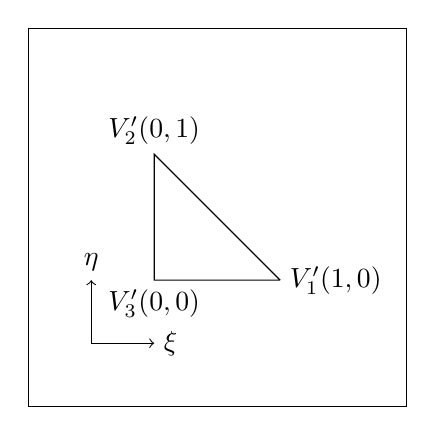
\begin{tikzpicture}[scale=0.8]
  \draw (-1,-1) -- (5,-1) -- (5,5) -- (-1,5) -- (-1,-1) ;
  \draw (3,1) node[right] {$V'_1(1,0)$} -- (1,3) node[above] {$V'_2(0,1)$} -- (1,1) node[below] {$V'_3(0,0)$} -- (3,1) ;
  \draw[->] (0,0) -- (1,0) node[right] {$\xi$} ;
  \draw[->] (0,0) -- (0,1) node[above] {$\eta$} ;
\end{tikzpicture}
\caption{
  The triangular element $K$ in the computaional domain
  is shown on the left
  while its reference element $K'$ 
  is shown on the right.
  }
\label{elems}
\end{figure}

\begin{figure}
\centering
\begin{tikzpicture}[scale=1.8]
  \draw (1,3) node[left] {$V_1$} -- (3,2) node[below] {$V_2$} -- (4,4) node[right] {$V_3$} -- (1,3) ;
  \draw (8/3,3) node[above] {$O$} -- (1,3) ;
  \draw (8/3,3) -- (3,2) ;
  \draw (8/3,3) -- (4,4) ;
  \draw[->] (0,0) -- (1,0) node[right] {$x$} ;
  \draw[->] (0,0) -- (0,1) node[above] {$y$} ;
\end{tikzpicture}
\caption{
  To define parameters $\xi$ and $\eta$
  we form three triangles
  $OV_2V_3$, $OV_3V_1$, and $OV_1V_2$
  which put together form the triangle $V_1V_2V_3$.
  }
\label{bary}
\end{figure}

Given a function $f(x,y): \mathbb{R}^2 \rightarrow \mathbb{R}$,
we need to find
\begin{align}
  \int_K f(x,y) dxdy \label{intK}
\end{align}
where K
is the triangular element
defined by the vertices
$V_1(x_1,y_1)$, $V_2(x_2,y_2)$ and $V_3(x_3,y_3)$
as seen in figure \ref{elems}.

\section{Transformation of coordinates}

As we have to consider points inside the triangular element
we switch to a different coordinate system (barycentric?).
As seen in figure \ref{bary},
given a point $O$ inside the triangle $V_1V_2V_3$,
we define
\begin{align*}
  \xi &= \frac{\text{area}(OV_2V_3)}{\text{area}(V_1V_2V_3)} \\
  \eta &= \frac{\text{area}(OV_1V_3)}{\text{area}(V_1V_2V_3)} \\
\end{align*}
Now, the points inside or on the triangle
are easily parameterised by $\xi$ and $\eta$
in the following manner.
\begin{align}
  x &= x_1 \xi + x_2 \eta + x_3 (1 - \xi - \eta) \label{x}\\
  y &= y_1 \xi + y_2 \eta + y_3 (1 - \xi - \eta) \label{y}
\end{align}
The tranformation from the parameters $(\xi,\eta)$
to $(x,y)$ is given by the following linear relation.
\begin{align}
  \begin{bmatrix} x \\ y \end{bmatrix} =
  \begin{bmatrix}
    x_1 - x_3 & x_2 - x_3 \\
    y_1 - y_3 & y_2 - y_3 \\
  \end{bmatrix}
  \begin{bmatrix} \xi \\ \eta \end{bmatrix}
  + \begin{bmatrix} x_3 \\ y_3 \end{bmatrix}
  \label{xy}
\end{align}
To transform the integral given in equation \ref{intK},
in terms of $\xi$ and $\eta$,
we have the following considerations.
\begin{description}
\item[Limits]
  We can see that
  $(\xi = 1, \eta = 0)$,
  $(\xi = 0, \eta = 1)$ and
  $(\xi = 0, \eta = 0)$
  correspond to the vertices
  $V_1$, $V_2$ and $V_3$ respectively
  as shown in figure \ref{elems}.
  Since, this mapping is linear we can conclude that
  the limits of the integration in equation \ref{intK}
  would be $\xi$ going from 0 to 1
  and $\eta$ going from 0 to $1 - \xi$.

\item[Integrand]
  The integrand $f(x,y)$
  will be written as $f(x(\xi,\eta), y(\xi,\eta)$
  using equations \ref{x} and \ref{y}.

\item[Infinitesimal area element]
  Small changes in $(x,y)$
  due to small change $(\delta \xi, \delta \eta)$ in $(\xi,\eta)$
  can be found by using equation \ref{xy}.
  \begin{align*}
    \begin{bmatrix} \delta x \\ \delta y \end{bmatrix} =
    J \begin{bmatrix} \delta \xi \\ \delta \eta \end{bmatrix}
  \end{align*}
  where
  \begin{align*}
    J = \begin{bmatrix}
      x_1 - x_3 & x_2 - x_3 \\
      y_1 - y_3 & y_2 - y_3 \\
    \end{bmatrix}
  \end{align*}
  Therefore the infinitesimal area element $dxdy$
  will have to be replaced by $\det (J) d\xi d\eta$.
  Fore more details regarding this refer to section \ref{det}.
\end{description}

\section{Integration in the reference element}

\section{On scaling and determinants \label{det}}

\end{document}


